\chapter{Evaluation}
The design of each strategy and the backtesting system allow for extensive parameterization, providing multiple axes for analysis. Parameters that can be adjusted are at what number of standard deviations away from the mean spread should a threshold set and a signal to be generated, how the trades are executed, limits on how much gas price should be when executing a trade, and also the volume of the initial investment. These are all factors that can effect the returns of the trading strategy. In the following sections, we will examine the performance of the strategy by varying these parameters, providing valuable insights into their influence on trading outcomes. For the purpose of data visualisation we denote the liquidity pool pairs by their index:
\begin{table}[!ht]
    \centering
    \begin{adjustwidth}{-0.5in}{-0.9in}
        \begin{tabular}{|p{20em}|p{20em}|p{3em}|}\hline
            Pool1 & Pool2 & Label\\\hline
            \truncate{20em}{USDC\_WETH\_0x88e6a0c2ddd26feeb64f039a2c41296fcb3f5640} & \truncate{20em}{USDC\_WETH\_0xe0554a476a092703abdb3ef35c80e0d76d32939f} & 0\\\hline
            \truncate{20em}{USDC\_WETH\_0x8ad599c3a0ff1de082011efddc58f1908eb6e6d8} & \truncate{20em}{USDC\_WETH\_0xe0554a476a092703abdb3ef35c80e0d76d32939f} & 1\\\hline
            \truncate{20em}{WETH\_USDT\_0x11b815efb8f581194ae79006d24e0d814b7697f6} & \truncate{20em}{USDC\_WETH\_0xe0554a476a092703abdb3ef35c80e0d76d32939f} & 2\\\hline
            \truncate{20em}{WETH\_USDT\_0x4e68ccd3e89f51c3074ca5072bbac773960dfa36} & \truncate{20em}{USDC\_WETH\_0xe0554a476a092703abdb3ef35c80e0d76d32939f} & 3\\\hline
            \truncate{20em}{DAI\_WETH\_0x60594a405d53811d3bc4766596efd80fd545a270} & \truncate{20em}{USDC\_WETH\_0xe0554a476a092703abdb3ef35c80e0d76d32939f} & 4\\\hline
            \truncate{20em}{DAI\_WETH\_0xc2e9f25be6257c210d7adf0d4cd6e3e881ba25f8} & \truncate{20em}{USDC\_WETH\_0xe0554a476a092703abdb3ef35c80e0d76d32939f} & 5\\\hline
            \truncate{20em}{USDC\_WETH\_0xe0554a476a092703abdb3ef35c80e0d76d32939f} & \truncate{20em}{WETH\_USDT\_0xc5af84701f98fa483ece78af83f11b6c38aca71d} & 6\\\hline
        \end{tabular}
    \end{adjustwidth}
    \caption{Liquidity pool pairs and their corresponding labels}
\end{table}
\vspace{-4ex}
\section{Number of Standard Deviations away from the Mean}
Varying the standard deviation in a mean reversion pairs trading strategy can have a significant impact on the strategy's returns. When the standard deviation threshold is set too high, it means that the spread between the pair's prices must deviate significantly from the mean before a signal is generated. In this case, the strategy may generate fewer trades, resulting in longer holding periods for positions, however this tends to have a greater return per trade. On the other hand, setting a lower standard deviation threshold makes the strategy more sensitive to smaller deviations from the mean. This increases the frequency of trade signals and potentially leads to more active trading. However, it also exposes the strategy to a higher risk of false signals or trading on noise in the price data. It can result in higher transaction costs and potentially lower returns due to increased trading activity, potentially resulting in losses.
\\[5mm]
Table \ref{tab:varying_sigma} displays the returns as the standard deviations away from the mean the threshold is set. For the purpose of this experiment the other parameters were; 100 ETH worth of initial investment, the window size set to 30 days, a gas price threshold of 1 ETH (i.e. not having a threshold), the interactions with the blockchain to be seperately executed and finally the lag that the lagged strategy uses is set to 1 hour. The period that trading occurs is from 18th December 2021 to 9th June 2023.
\\[5mm]
We can see that as $\sigma \rightarrow 0$, the number of trades increases however causes the returns to be more negative (and in some cases terminating early with 100\% loss) than positive, likely due to trades being opened when gas fees are substantially larger than the profit. However, if $\sigma$ is larger, although the profits from each trade increases, the number of opportunities that were actionable were limited. Another interesting feature that can easily be spotted is that the Constant Hedge Ratio Strategy makes little to no profit in all cases whereas the other strategies perform better as $\sigma \rightarrow \sim2$. Furthermore, all of the strategies return a profit on pool pair 6 with the exception of the Kalman Filter Strategy, albeit with a higher threshold.
\\[5mm]
Consistent profit among all of the pool pairs, excluding pool pair 6, is also achieved at different $\sigma$s. We can see in Figure \ref{fig:varyStd} that the average return across all liquidity pool pairs that each strategy generates at each standard deviation. The Kalman Filter becomes largely profitable at $\sigma = 0.5$, whereas the lagged, sliding window and granger causality strategies become profitable at $\sigma = 2$. This is highly due to the fact that the Kalman Filter is better able to find underlying trends thus being better at selecting the hedge ratio.

\definecolor{green}{RGB}{0,153,0}
\begin{table}[!ht]
    \centering
    \begin{adjustwidth}{-0.8in}{-0.9in}
        \begin{tabular}{|p{4em}|p{2em}|p{3em}|p{3em}|p{3em}|p{3em}|p{3em}|p{3em}|p{3em}|p{3em}|p{3em}|p{3em}|}\hline
            Std & Pool Pair & \multicolumn{10}{|c|}{Strategy's Return} \\\cline{3-12}
            &   & \multicolumn{2}{|c|}{Constant} & \multicolumn{2}{|c|}{Sliding Window} & \multicolumn{2}{|c|}{Lagged} & \multicolumn{2}{|c|}{Granger Causality} & \multicolumn{2}{|c|}{Kalman Filter}\\\cline{3-12}
            & & Return \% & \# of Trades & Return \% & \# of Trades & Return \% & \# of Trades & Return \% & \# of Trades & Return \% & \# of Trades\\\hline
            
            & 0 & \textcolor{green}{5.44} & 360 & \textcolor{green}{29.28} & 661 & \textcolor{green}{66.29} & 687 & \textcolor{green}{20.92} & 715 & \textcolor{red}{-100} & 70\\\cline{3-12}
            & 1 & \textcolor{red}{-100} & 104 & \textcolor{red}{-83.7} & 660 & \textcolor{red}{-77.28} & 653 & \textcolor{red}{-84.93} & 681 & \textcolor{red}{-100} & 71\\\cline{3-12}
            & 2 & \textcolor{green}{5.83} & 454 & \textcolor{red}{-2.1} & 634 & \textcolor{green}{43.6} & 619 & \textcolor{green}{20.12} & 659 & \textcolor{green}{89.13} & 236\\\cline{3-12}
            $\sigma=0.1$& 3 & \textcolor{red}{-67.51} & 535 & \textcolor{red}{-70.51} & 572 & \textcolor{red}{-73.24} & 604 & \textcolor{red}{-91.67} & 714 & \textcolor{red}{-100} & 74\\\cline{3-12}
            & 4 & \textcolor{green}{11.14} & 375 & \textcolor{green}{10.06} & 759 & \textcolor{green}{58.61} & 669 & \textcolor{green}{12.3} & 742 & \textcolor{red}{-100} & 70\\\cline{3-12}
            & 5 & \textcolor{red}{-53.44} & 396 & \textcolor{red}{-75.16} & 587 & \textcolor{red}{-68.27} & 593 & \textcolor{red}{-100} & 599 & \textcolor{red}{-100} & 71\\\cline{3-12}
            & 6 & \textcolor{red}{-100} & 26 & \textcolor{red}{-82.0} & 213 & \textcolor{red}{-76.2} & 198 & \textcolor{red}{-72.16} & 190 & \textcolor{red}{-100} & 27\\\hline\hline
            
            & 0 & \textcolor{green}{11.77} & 723 & \textcolor{red}{-15.81} & 1223 & \textcolor{green}{104.48} & 1185 & \textcolor{red}{-8.34} & 1228 & \textcolor{green}{241.96} & 378\\\cline{3-12}
            & 1 & \textcolor{red}{-100} & 832 & \textcolor{red}{-100} & 920 & \textcolor{red}{-100} & 936 & \textcolor{red}{-100} & 989 & \textcolor{green}{60.2} & 456\\\cline{3-12}
            & 2 & \textcolor{green}{9.19} & 688 & \textcolor{red}{-0.88} & 1105 & \textcolor{green}{124.82} & 1025 & \textcolor{green}{10.14} & 1067 & \textcolor{green}{295.01} & 396\\\cline{3-12}
            $\sigma=0.5$& 3 & \textcolor{red}{-93.51} & 794 & \textcolor{red}{-100} & 944 & \textcolor{red}{-92.35} & 1063 & \textcolor{red}{-100} & 672 & \textcolor{green}{37.63} & 425\\\cline{3-12}
            & 4 & \textcolor{green}{26.01} & 826 & \textcolor{red}{-16.12} & 1243 & \textcolor{green}{112.45} & 1213 & \textcolor{green}{13.72} & 1237 & \textcolor{green}{244.51} & 391\\\cline{3-12}
            & 5 & \textcolor{red}{-95.02} & 837 & \textcolor{red}{-100} & 854 & \textcolor{red}{-100} & 905 & \textcolor{red}{-100} & 851 & \textcolor{green}{90.57} & 388\\\cline{3-12}
            & 6 & \textcolor{red}{-100} & 40 & \textcolor{red}{-96.69} & 359 & \textcolor{red}{-84.14} & 301 & \textcolor{red}{-96.34} & 372 & \textcolor{red}{-100} & 61\\\hline\hline
            
            & 0 & \textcolor{red}{-21.41} & 675 & \textcolor{red}{-1.59} & 864 & \textcolor{green}{129.7} & 865 & \textcolor{green}{52.74} & 873 & \textcolor{green}{164.34} & 442\\\cline{3-12}
            & 1 & \textcolor{red}{-100} & 791 & \textcolor{red}{-100} & 814 & \textcolor{red}{-93.81} & 1022 & \textcolor{red}{-100} & 829 & \textcolor{red}{-10.31} & 505\\\cline{3-12}
            & 2 & \textcolor{red}{-21.23} & 535 & \textcolor{green}{7.04} & 777 & \textcolor{green}{150.19} & 721 & \textcolor{green}{62.07} & 714 & \textcolor{green}{184.32} & 404\\\cline{3-12}
            $\sigma=1$& 3 & \textcolor{red}{-100} & 497 & \textcolor{red}{-100} & 657 & \textcolor{red}{-74.92} & 872 & \textcolor{red}{-94.72} & 859 & \textcolor{green}{1.9} & 436\\\cline{3-12}
            & 4 & \textcolor{red}{-5.26} & 689 & \textcolor{green}{15.54} & 799 & \textcolor{green}{156.04} & 822 & \textcolor{green}{58.94} & 822 & \textcolor{green}{190.11} & 460\\\cline{3-12}
            & 5 & \textcolor{red}{-100} & 533 & \textcolor{red}{-100} & 612 & \textcolor{red}{-69.44} & 785 & \textcolor{red}{-87.97} & 769 & \textcolor{green}{37.38} & 408\\\cline{3-12}
            & 6 & \textcolor{red}{-53.08} & 108 & \textcolor{red}{-66.08} & 169 & \textcolor{red}{-46.79} & 125 & \textcolor{red}{-59.38} & 159 & \textcolor{red}{-41.59} & 158\\\hline\hline
            
            & 0 & \textcolor{green}{5.7} & 365 & \textcolor{green}{48.67} & 447 & \textcolor{green}{144.27} & 476 & \textcolor{green}{37.48} & 483 & \textcolor{green}{178.36} & 179\\\cline{3-12}
            & 1 & \textcolor{red}{-100} & 408 & \textcolor{red}{-63.97} & 509 & \textcolor{red}{-30.62} & 504 & \textcolor{red}{-65.49} & 510 & \textcolor{green}{68.75} & 221\\\cline{3-12}
            & 2 & \textcolor{red}{-6.09} & 302 & \textcolor{green}{22.37} & 402 & \textcolor{green}{115.76} & 391 & \textcolor{green}{30.37} & 383 & \textcolor{green}{171.74} & 147\\\cline{3-12}
            $\sigma=1.5$& 3 & \textcolor{red}{-71.49} & 389 & \textcolor{red}{-58.55} & 453 & \textcolor{red}{-27.34} & 449 & \textcolor{red}{-64.5} & 456 & \textcolor{green}{79.79} & 166\\\cline{3-12}
            & 4 & \textcolor{red}{-12.11} & 324 & \textcolor{green}{38.58} & 428 & \textcolor{green}{128.86} & 426 & \textcolor{green}{31.11} & 433 & \textcolor{green}{176.14} & 201\\\cline{3-12}
            & 5 & \textcolor{red}{-100} & 312 & \textcolor{red}{-51.69} & 402 & \textcolor{red}{-2.83} & 379 & \textcolor{red}{-46.45} & 386 & \textcolor{green}{88.52} & 175\\\cline{3-12}
            & 6 & \textcolor{red}{-42.58} & 77 & \textcolor{red}{-40.18} & 87 & \textcolor{red}{-39.6} & 89 & \textcolor{red}{-32.74} & 83 & \textcolor{red}{-18.52} & 102\\\hline\hline
            
            & 0 & \textcolor{red}{-10.35} & 288 & \textcolor{green}{38.26} & 342 & \textcolor{green}{141.77} & 353 & \textcolor{green}{46.07} & 359 & \textcolor{green}{175.37} & 153\\\cline{3-12}
            & 1 & \textcolor{red}{-67.13} & 358 & \textcolor{red}{-29.23} & 293 & \textcolor{red}{-7.71} & 323 & \textcolor{red}{-36.45} & 320 & \textcolor{green}{74.13} & 178\\\cline{3-12}
            & 2 & \textcolor{red}{-2.51} & 225 & \textcolor{green}{33.15} & 277 & \textcolor{green}{115.65} & 270 & \textcolor{green}{47.41} & 264 & \textcolor{green}{167.95} & 133\\\cline{3-12}
            $\sigma=1.75$& 3 & \textcolor{red}{-59.62} & 309 & \textcolor{red}{-21.28} & 268 & \textcolor{red}{-1.49} & 294 & \textcolor{red}{-20.76} & 266 & \textcolor{green}{88.24} & 145\\\cline{3-12}
            & 4 & \textcolor{red}{-3.72} & 241 & \textcolor{green}{41.37} & 294 & \textcolor{green}{92.24} & 291 & \textcolor{green}{34.18} & 289 & \textcolor{green}{146.99} & 152\\\cline{3-12}
            & 5 & \textcolor{red}{-54.88} & 287 & \textcolor{red}{-14.02} & 225 & \textcolor{green}{14.77} & 250 & \textcolor{red}{-17.77} & 237 & \textcolor{green}{103.61} & 152\\\cline{3-12}
            & 6 & \textcolor{red}{-47.31} & 76 & \textcolor{red}{-26.89} & 67 & \textcolor{red}{-40.81} & 76 & \textcolor{red}{-30.3} & 55 & \textcolor{red}{-22.66} & 74\\\hline\hline
            
            & 0 & \textcolor{green}{2.11} & 226 & \textcolor{green}{44.05} & 271 & \textcolor{green}{90.62} & 268 & \textcolor{green}{50.97} & 273 & \textcolor{green}{108.12} & 116\\\cline{3-12}
            & 1 & \textcolor{red}{-41.61} & 245 & \textcolor{green}{7.67} & 165 & \textcolor{green}{30.12} & 184 & \textcolor{green}{4.58} & 183 & \textcolor{green}{57.28} & 125\\\cline{3-12}
            & 2 & \textcolor{red}{-8.64} & 191 & \textcolor{green}{45.26} & 190 & \textcolor{green}{90.81} & 202 & \textcolor{green}{46.24} & 195 & \textcolor{green}{98.06} & 106\\\cline{3-12}
            $\sigma=2$& 3 & \textcolor{red}{-48.82} & 228 & \textcolor{green}{5.81} & 160 & \textcolor{green}{24.92} & 178 & \textcolor{green}{3.07} & 172 & \textcolor{green}{57.92} & 121\\\cline{3-12}
            & 4 & \textcolor{green}{8.74} & 206 & \textcolor{green}{45.91} & 190 & \textcolor{green}{85.04} & 201 & \textcolor{green}{46.03} & 204 & \textcolor{green}{96.82} & 125\\\cline{3-12}
            & 5 & \textcolor{red}{-27.79} & 192 & \textcolor{green}{10.78} & 138 & \textcolor{green}{32.9} & 147 & \textcolor{green}{4.63} & 144 & \textcolor{green}{69.22} & 125\\\cline{3-12}
            & 6 & \textcolor{red}{-37.31} & 65 & \textcolor{red}{-22.0} & 49 & \textcolor{red}{-24.93} & 54 & \textcolor{red}{-19.06} & 44 & \textcolor{green}{0.99} & 53\\\hline\hline
            
            & 0 & \textcolor{green}{2.59} & 54 & \textcolor{green}{28.73} & 102 & \textcolor{green}{26.55} & 83 & \textcolor{green}{18.26} & 90 & \textcolor{green}{27.46} & 51\\\cline{3-12}
            & 1 & \textcolor{red}{-5.71} & 64 & \textcolor{green}{21.12} & 49 & \textcolor{green}{18.19} & 46 & \textcolor{green}{15.78} & 49 & \textcolor{green}{23.33} & 60\\\cline{3-12}
            & 2 & \textcolor{green}{1.95} & 61 & \textcolor{green}{20.39} & 56 & \textcolor{green}{22.55} & 64 & \textcolor{green}{14.16} & 61 & \textcolor{green}{21.34} & 52\\\cline{3-12}
            $\sigma=3$& 3 & \textcolor{red}{-10.22} & 73 & \textcolor{green}{12.31} & 46 & \textcolor{green}{11.0} & 48 & \textcolor{green}{7.19} & 47 & \textcolor{green}{12.46} & 58\\\cline{3-12}
            & 4 & \textcolor{green}{4.65} & 67 & \textcolor{green}{32.37} & 57 & \textcolor{green}{28.98} & 64 & \textcolor{green}{26.74} & 68 & \textcolor{green}{26.45} & 57\\\cline{3-12}
            & 5 & \textcolor{red}{-6.49} & 53 & \textcolor{green}{20.89} & 39 & \textcolor{green}{18.45} & 39 & \textcolor{green}{13.37} & 42 & \textcolor{green}{26.67} & 57\\\cline{3-12}
            & 6 & \textcolor{red}{-1.72} & 13 & \textcolor{red}{-4.74} & 20 & \textcolor{red}{-3.19} & 25 & \textcolor{red}{-2.39} & 19 & \textcolor{green}{12.01} & 16\\\hline
        \end{tabular}
    \end{adjustwidth}
    \caption{Returns of various standard deviation thresholds of each strategy \label{tab:varying_sigma}}.
\end{table}

\begin{figure}[h!]
    \centering
    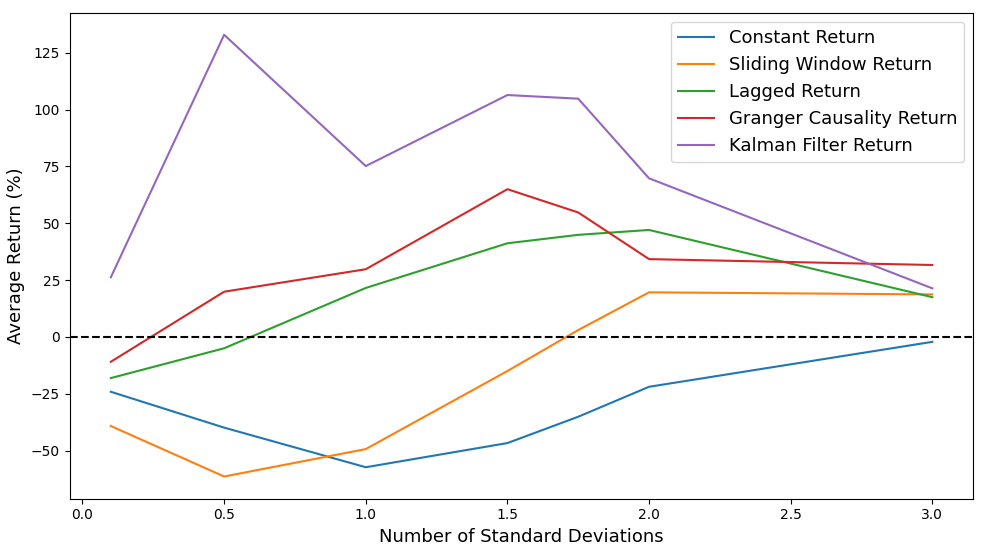
\includegraphics[width=0.8\textwidth]{evaluation/Images/VaryStd.png}
    \caption{Plot of Average Return across all pool pairs by the standard deviation}
    \label{fig:varyStd}
\end{figure}

\section{Initial Investment Volume}

\section{Window Size}

\section{Fees}
\subsection{Batched Transactions vs Seperately Executed Transactions}
\subsection{Gas Fee Threshold}

\section{Beta}

\section{Sharpe Ratio}

\section{Comparison with Other results}
